\documentclass[11pt,a4paper]{article}

\usepackage[margin=1.7cm]{geometry}
\usepackage{fontspec}
\usepackage{longtable}
\usepackage{array}
\usepackage{tikz}
\usetikzlibrary{arrows.meta}

\setmainfont{Noto Serif CJK TC}
\setsansfont{Noto Sans CJK TC}
\setmonofont{DejaVu Sans Mono}
\setlength{\parindent}{0pt}
\setlength{\LTleft}{0pt}
\setlength{\LTright}{0pt}

\newcommand{\dpath}[1]{{\footnotesize\texttt{\detokenize{#1}}}}
% This TeX installation has no CJK line-breaking package. Mark natural
% break points in the long table descriptions with this command.
\newcommand{\cjkbreak}{\allowbreak}

\begin{document}
\documentclass[11pt,a4paper]{article}

\usepackage[margin=1.7cm]{geometry}
\usepackage{fontspec}
\usepackage{longtable}
\usepackage{array}
\usepackage{tikz}
\usetikzlibrary{arrows.meta}

\setmainfont{Noto Serif CJK TC}
\setsansfont{Noto Sans CJK TC}
\setmonofont{DejaVu Sans Mono}
\setlength{\parindent}{0pt}
\setlength{\LTleft}{0pt}
\setlength{\LTright}{0pt}

\newcommand{\dpath}[1]{{\footnotesize\texttt{\detokenize{#1}}}}
% This TeX installation has no CJK line-breaking package. Mark natural
% break points in the long table descriptions with this command.
\newcommand{\cjkbreak}{\allowbreak}

\begin{document}

\section*{資料流程框架}

\begin{center}
\begin{tikzpicture}[
  >=Latex,
  flow/.style={->, thick},
  stage/.style={draw, rounded corners, align=center, text width=7.3cm,
    minimum height=0.82cm, inner sep=4pt, font=\small},
  side/.style={draw, rounded corners, align=center, text width=4.15cm,
    minimum height=0.82cm, inner sep=4pt, font=\small}
]
  \node[stage] (proof) at (0,0) {執行 proof};
  \node[stage] (raw) at (0,-1.3)
    {\dpath{data/raw/}\\Collector 收集並限制保留的 records};
  \node[stage] (merged) at (0,-2.6)
    {\dpath{data/merged/}\\跨 proofs 合併同一個 tactic 的 records};
  \node[stage] (dedup) at (0,-3.9)
    {\dpath{data/dedup/}\\完全去重};
  \node[stage] (sampling) at (0,-5.2)
    {\dpath{data/sampling/}\\similarity check、各組配額與空缺遞補};
  \node[stage] (generation) at (0,-6.5)
    {\dpath{data/generation/}\\準備實際要送給 LLM 的 records 和 prompt};
  \node[stage] (descriptions) at (0,-7.8)
    {\dpath{llm_output/descriptions/}\\LLM 生成的 descriptions};
  \node[stage] (judge) at (0,-9.1)
    {\dpath{metrics/judge_responses/}\\LLM judge 的回答};
  \node[stage] (record) at (0,-10.4)
    {\dpath{metrics/record_scores/}\\將回答整理成逐筆分數};
  \node[stage] (tactic) at (0,-11.7)
    {\dpath{metrics/tactic_scores/}\\按 tactic／description 彙整};

  \node[side] (selection) at (6.4,-5.2)
    {\dpath{metrics/selection/}\\篩選決定與統計};
  \node[side] (evaluation) at (6.4,-7.8)
    {\dpath{data/evaluation/}\\選定用來評分的 records};

  \draw[flow] (proof) -- (raw);
  \draw[flow] (raw) -- (merged);
  \draw[flow] (merged) -- (dedup);
  \draw[flow] (dedup) -- (sampling);
  \draw[flow] (sampling) -- (generation);
  \draw[flow] (generation) -- (descriptions);
  \draw[flow] (descriptions) -- (judge);
  \draw[flow] (judge) -- (record);
  \draw[flow] (record) -- (tactic);
  \draw[flow] (sampling) -- (selection);
  \draw[flow] (evaluation.south) |- (judge.east);
\end{tikzpicture}
\end{center}

\small
\textbf{跨階段追溯：}\dpath{data/metadata/} 記錄上述各階段的來源、設定與檔案關係。

\clearpage
\section*{各階段資料夾說明}

\setlength{\tabcolsep}{4pt}
\renewcommand{\arraystretch}{1.35}
\begin{longtable}{|>{\raggedright\arraybackslash}p{1.7cm}|>{\raggedright\arraybackslash}p{4.6cm}|>{\raggedright\arraybackslash}p{10.1cm}|}
\hline
\textbf{順序} & \textbf{資料夾} & \textbf{裡面存什麼} \\ \hline
\endfirsthead
\hline
\textbf{順序} & \textbf{資料夾} & \textbf{裡面存什麼} \\ \hline
\endhead
1 & \dpath{data/raw/} & Collector 跑完 proof 後輸出的 records。\cjkbreak 已經受到 collector 的大小、容量與選取規則限制，\cjkbreak 因此不是執行過程中的所有 records。 \\ \hline
2 & \dpath{data/merged/} & 把不同 proofs 中同一個 tactic 的候選 records 集合在一起，\cjkbreak 此階段仍可包含重複資料。 \\ \hline
3 & \dpath{data/dedup/} & 依既有 record identity 規則，\cjkbreak 移除完全重複後的 records。\cjkbreak 尚未做後面的 similarity 與最終配額選擇。 \\ \hline
4 & \dpath{data/sampling/} & 經過 similarity check、分組配額與遞補後，\cjkbreak 最後選出的 records，\cjkbreak 供 description generation 使用。 \\ \hline
4 的紀錄 & \dpath{metrics/selection/} & 為什麼保留或排除某筆 record、相似度比較、\cjkbreak 各組數量與篩選設定。\cjkbreak 這不是 LLM 對 description 的評分。 \\ \hline
5 & \dpath{data/generation/} & 實際生成請求：\cjkbreak 包含送進 LLM 的 records、prompt 和相關設定。\cjkbreak 若生成時另外抽樣或截斷，\cjkbreak 這裡記錄實際使用的版本。 \\ \hline
6 & \dpath{llm_output/descriptions/} & LLM 產生的 descriptions，\cjkbreak 以及生成嘗試與狀態等紀錄。 \\ \hline
7 & \dpath{data/evaluation/} & Judge 使用的 records、\cjkbreak 候選 descriptions 的對應資訊與評分任務。\cjkbreak 放在這裡不代表它們與生成資料沒有重疊，\cjkbreak 是否獨立要看實驗設計。 \\ \hline
8 & \dpath{metrics/judge_responses/} & 保存 judge 的回答，\cjkbreak 包括逐筆判斷、理由、用量和呼叫錯誤。 \\ \hline
9 & \dpath{metrics/record_scores/} & 把有效回答整理成每筆 record 對每份 description 的分數與理由。\cjkbreak 目前這個 judge 的對應是 full=1、partial=0.5、none=0。 \\ \hline
10 & \dpath{metrics/tactic_scores/} & 將逐筆分數彙整成每個 tactic／description 的結果，\cjkbreak 供比較、報表與表格使用。 \\ \hline
全流程 & \dpath{data/metadata/} & s2n-bignum commit、實驗設定、來源檔案、雜湊、搬移對照等追溯資訊。\cjkbreak 各資料清單的 index 也可以與 records 放在同一階段資料夾。 \\ \hline
\end{longtable}

\end{document}

% Design note based on the discussion on 2026-10-15; not an experiment report.
% Section fragment: include inside an existing document with
% % Design note based on the discussion on 2026-10-15; not an experiment report.
% Section fragment: include inside an existing document with
% % Design note based on the discussion on 2026-10-15; not an experiment report.
% Section fragment: include inside an existing document with
% \input{sampling-training-evaluation-workflows}
% Needs Chinese-capable fonts, tikz, and \usetikzlibrary{arrows.meta}.
% The existing framework.tex already provides these prerequisites.

\section{比較兩階段 sampling 時的 training 與 evaluation 切分}
\label{sec:sampling-training-evaluation-workflows}

本節記錄預定的實驗設計，\allowbreak 不代表已經實作或執行。
這裡的 training records 是提供給 LLM 生成 description 的範例，\allowbreak
不會訓練或更新模型權重。
為避免混淆，\allowbreak 下文區分「training 候選池」與「最後送進 LLM 的 generation list」。

\begin{itemize}
  \item \textbf{第一次 sampling：}collector 在 proof 執行時選取並保留候選 records。
  \item \textbf{中間處理：}依既定流程合併候選、exact dedup 與 similarity check。
  \item \textbf{第二次 sampling：}從候選池依分組配額與遞補規則，\allowbreak
        選出最後用來生成 description 的 records。
\end{itemize}

\subsection{情況一：比較第一次 sampling 方法}
\label{subsec:holdout-first-sampling}

A、B 從相同 proof 與 source commit 開始，\allowbreak
使用不同的第一次 sampling 方法。
兩邊使用相同候選容量，\allowbreak 並固定其餘 collector 設定、dedup 與 similarity check 規則。
因此，中間處理後的候選 lists 可以不同，\allowbreak 這正是要保留的實驗差異。

\begin{center}
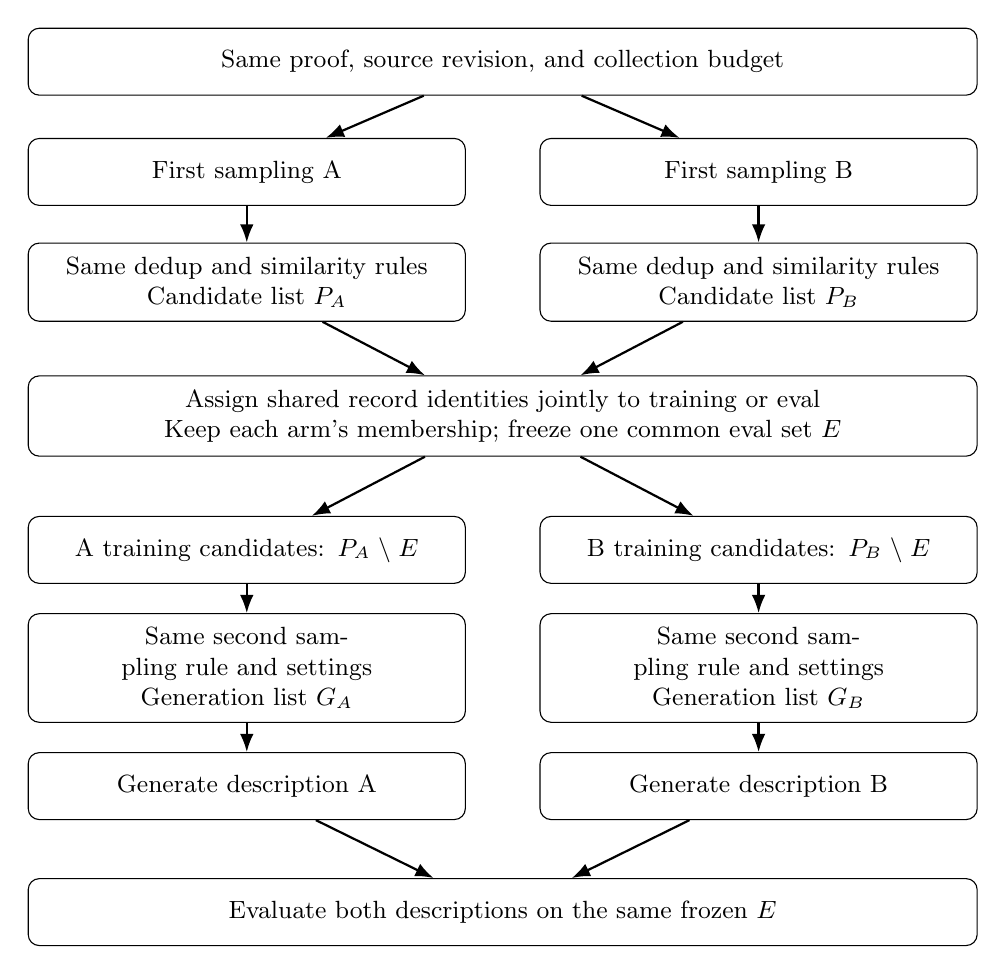
\begin{tikzpicture}[
  >=Latex,
  flow/.style={->, thick},
  box/.style={draw, rounded corners, align=center, text width=5.2cm,
    minimum height=0.85cm, inner sep=5pt, font=\small},
  wide/.style={box, text width=11.7cm}
]
  \node[wide] (proof) at (0,0) {Same proof, source revision, and collection budget};
  \node[box] (firsta) at (-3.25,-1.4) {First sampling A};
  \node[box] (firstb) at (3.25,-1.4) {First sampling B};
  \node[box] (poola) at (-3.25,-2.8) {Same dedup and similarity rules\\Candidate list $P_A$};
  \node[box] (poolb) at (3.25,-2.8) {Same dedup and similarity rules\\Candidate list $P_B$};
  \node[wide] (split) at (0,-4.5) {Assign shared record identities jointly to training or eval\\Keep each arm's membership; freeze one common eval set $E$};
  \node[box] (traina) at (-3.25,-6.2) {A training candidates: $P_A\setminus E$};
  \node[box] (trainb) at (3.25,-6.2) {B training candidates: $P_B\setminus E$};
  \node[box] (seconda) at (-3.25,-7.7) {Same second sampling rule and settings\\Generation list $G_A$};
  \node[box] (secondb) at (3.25,-7.7) {Same second sampling rule and settings\\Generation list $G_B$};
  \node[box] (desca) at (-3.25,-9.2) {Generate description A};
  \node[box] (descb) at (3.25,-9.2) {Generate description B};
  \node[wide] (judge) at (0,-10.8) {Evaluate both descriptions on the same frozen $E$};
  \draw[flow] (proof) -- (firsta);
  \draw[flow] (proof) -- (firstb);
  \draw[flow] (firsta) -- (poola);
  \draw[flow] (firstb) -- (poolb);
  \draw[flow] (poola) -- (split);
  \draw[flow] (poolb) -- (split);
  \draw[flow] (split) -- (traina);
  \draw[flow] (split) -- (trainb);
  \draw[flow] (traina) -- (seconda);
  \draw[flow] (trainb) -- (secondb);
  \draw[flow] (seconda) -- (desca);
  \draw[flow] (secondb) -- (descb);
  \draw[flow] (desca) -- (judge);
  \draw[flow] (descb) -- (judge);
\end{tikzpicture}
\end{center}

\paragraph{一起決定歸屬，不是混合兩邊的生成資料。}
一起查看 A、B 的候選，是為了辨認內容相同的 records，\allowbreak
統一決定它們是否屬於 evaluation。
若某筆 record 被選入共同 eval set，\allowbreak 必須從兩邊的 training 候選中排除。
不能將 B 獨有的 record 加進 A，\allowbreak 或反過來補入。
A training 與 B training 可以互相重疊，\allowbreak 但任一方都不能與 eval 重疊。

例如，下列編號代表依內容辨認的 record identity，\allowbreak 而不是檔案內的行號：
\begin{quote}
$P_A=\{r_1,r_2,r_3,r_4\}$，$P_B=\{r_2,r_3,r_5,r_6\}$。\\
若選定 $E=\{r_3,r_5\}$，則\\
A training 為 $\{r_1,r_2,r_4\}$；\\
B training 為 $\{r_2,r_6\}$。
\end{quote}
兩份 descriptions 都評 $E$，\allowbreak 即使其中的 $r_5$ 原本只存在於 B 候選池。
共同 eval 不限於 A、B 的交集，\allowbreak 但每個內容 identity 只保留一份。

\paragraph{控制最後送進 LLM 的筆數。}
在相同 tactic 內，\allowbreak 對 success 與 failure 分開決定共同的生成筆數：
\[
  n_{t,o}=\min\bigl(K_{t,o},\ |T_{A,t,o}|,\ |T_{B,t,o}|\bigr),
\]
其中 $t$ 表示 tactic，\allowbreak $o$ 表示 success 或 failure，\allowbreak
$T$ 是移除 eval 後的 training 候選，\allowbreak $K$ 是預定的生成上限。
兩邊各自用相同的 deterministic 第二次 sampling 規則選出 $n_{t,o}$ 筆。
這個設計對齊的是每個 tactic 的 success／failure 總筆數，\allowbreak
不額外要求各 goal-count group 的實際筆數都相同。
相同筆數也不代表相同 token 數或 LLM 費用。
若某個 outcome 在任一邊沒有 training 候選，\allowbreak
對齊後兩邊該 outcome 都使用零筆；\allowbreak 應明確記錄此限制。

例如，若 success 上限為 40，\allowbreak
兩邊可用候選分別為 35 與 28，\allowbreak 最後各選 28 筆。
較多的一方不必刪除其餘已保存候選；\allowbreak 它們只是未用於這輪生成。
這是\textbf{固定生成筆數的比較}，\allowbreak 不是讓每種方法用盡所有可用資料的比較。

\paragraph{第一次先保留較大的候選池。}
若擔心切出 eval 後 training 太少，\allowbreak
可以在第一次 sampling 使用相同且較大的候選容量。
例如，兩邊先各保留 120 筆候選，\allowbreak
經過去重、similarity 與 eval 排除後，\allowbreak 再各選最多 40 筆 success。
這只是示例，\allowbreak 不是已決定的參數，也不保證每個 tactic 都有足夠資料。
先離線統計各階段保留量，\allowbreak 再決定容量與 eval 大小；\allowbreak
不能複製 records 湊數或將 eval 放回 training。
候選容量增加也會增加收集與儲存成本。

\subsection{情況二：比較第二次 sampling 方法}
\label{subsec:holdout-second-sampling}

第一次 sampling、dedup 與 similarity check 全部相同，\allowbreak
先取得一份共同候選池 $P$。
\textbf{在第二次 sampling 之前只切分一次}，\allowbreak
得到共同 training 候選池 $T$ 與固定 eval set $E$。
A、B 的第二次 sampling 都從同一份 $T$ 開始選。

\begin{center}
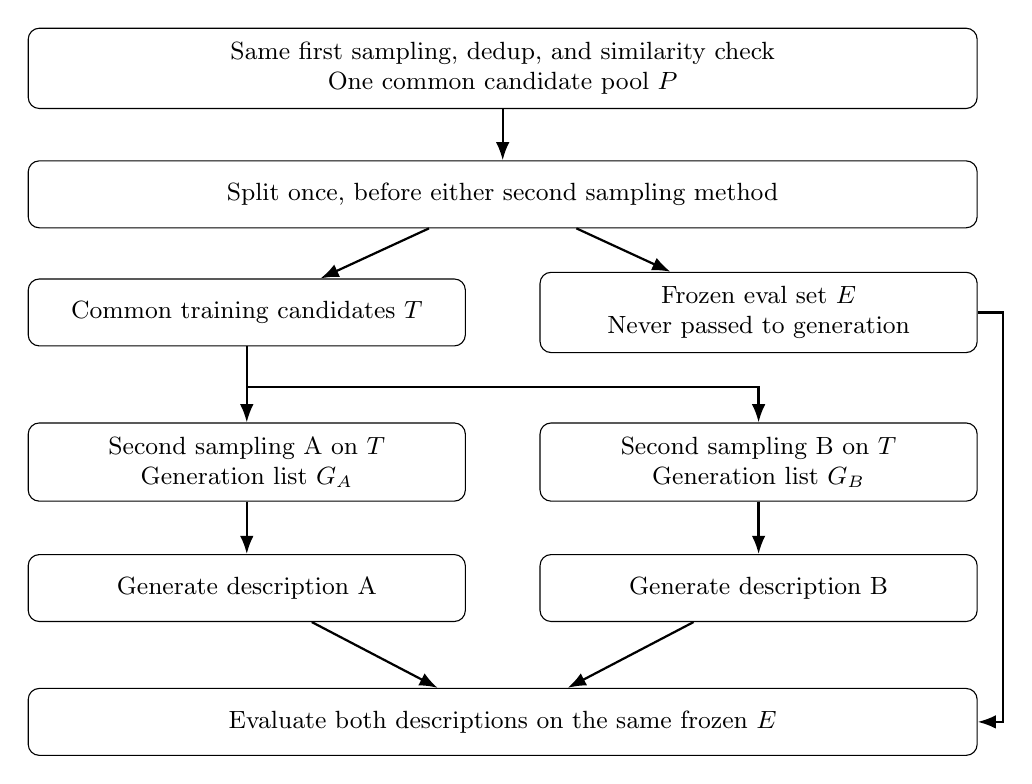
\begin{tikzpicture}[
  >=Latex,
  flow/.style={->, thick},
  box/.style={draw, rounded corners, align=center, text width=5.2cm,
    minimum height=0.85cm, inner sep=5pt, font=\small},
  wide/.style={box, text width=11.7cm}
]
  \node[wide] (pool) at (0,0) {Same first sampling, dedup, and similarity check\\One common candidate pool $P$};
  \node[wide] (split) at (0,-1.6) {Split once, before either second sampling method};
  \node[box] (training) at (-3.25,-3.1) {Common training candidates $T$};
  \node[box] (eval) at (3.25,-3.1) {Frozen eval set $E$\\Never passed to generation};
  \node[box] (seconda) at (-3.25,-5.0) {Second sampling A on $T$\\Generation list $G_A$};
  \node[box] (secondb) at (3.25,-5.0) {Second sampling B on $T$\\Generation list $G_B$};
  \node[box] (desca) at (-3.25,-6.6) {Generate description A};
  \node[box] (descb) at (3.25,-6.6) {Generate description B};
  \node[wide] (judge) at (0,-8.3) {Evaluate both descriptions on the same frozen $E$};
  \draw[flow] (pool) -- (split);
  \draw[flow] (split) -- (training);
  \draw[flow] (split) -- (eval);
  \draw[flow] (training) -- (seconda);
  \draw[flow] (training.south) -- (-3.25,-4.05) -- (3.25,-4.05) -- (secondb.north);
  \draw[flow] (seconda) -- (desca);
  \draw[flow] (secondb) -- (descb);
  \draw[flow] (desca) -- (judge);
  \draw[flow] (descb) -- (judge);
  \draw[flow] (eval.east) -- (6.35,-3.1) -- (6.35,-8.3) -- (judge.east);
\end{tikzpicture}
\end{center}

例如，共同候選池有 100 筆 success，\allowbreak
先保留 20 筆作為 eval，\allowbreak 剩下 80 筆作為 training 候選。
A、B 各自從同一份 80 筆候選選 40 筆，\allowbreak
生成兩份 descriptions，\allowbreak 然後都評同一份預留的 20 筆。
這些數字只是示意，\allowbreak failure 也需要另外規劃保留量。

不建議先執行第二次 sampling，\allowbreak
再從 A、B 的最終 lists 抽走 eval，\allowbreak 然後又 sampling 一次。
這會移除方法刻意保留的代表，\allowbreak
測到的變成兩輪選取與移除的整體效果。
若要單獨比較第二次選取方法，\allowbreak
應固定共同 training 候選、生成上限與非比較中的設定。
若某個方法因組別限制無法填滿共同目標，\allowbreak
須事先決定如何處理並記錄實際筆數，\allowbreak 不能默認兩邊一定選滿。

\subsection{兩種設計都必須遵守的規則}

令 $G_A$、$G_B$ 為實際送進 LLM 的 generation lists，\allowbreak
共同的無重疊要求為
\[
  G_A\cap E=\emptyset,\qquad G_B\cap E=\emptyset.
\]
不要求 $G_A\cap G_B=\emptyset$：\allowbreak
兩種方法可以選中相同的 training records。

\begin{enumerate}
  \item \textbf{按內容決定歸屬。}
        不能只比較檔名、proof 名稱或 record 編號。
        應依一致的內容 identity 規則辨認 records，\allowbreak
        並檢查生成與評分實際看到的 evidence 是否重複；\allowbreak
        僅來源 metadata 不同不能當成新的獨立案例。
  \item \textbf{先切分、固定，再生成與評分。}
        切分採 deterministic 規則，\allowbreak 保存 membership 與設定，\allowbreak
        不依生成結果或 judge 分數重新挑選 eval。
        切分比例、穩定排序規則、各 tactic／outcome 最低筆數仍待決定。
  \item \textbf{不足資料時明確記錄。}
        分別記錄各 tactic 的 success／failure 與 goal-count 分布。
        若沒有可評 records，\allowbreak 該項標記 N/A；\allowbreak
        若生成資料不足，\allowbreak 依事先約定的規則縮小規模或不納入，\allowbreak
        不把缺失資料當成零分。
  \item \textbf{固定生成與 judge 條件。}
        除了要比較的 sampling 方法，\allowbreak
        固定 prompt、模型、effort、token budget 與評分規則。
        兩份 descriptions 評同一份 eval evidence，\allowbreak
        分別呈現每個 tactic 的 success／failure 分數與筆數。
        Deterministic 選取不代表 LLM 回答必然相同。
  \item \textbf{保存每階段數量與來源。}
        保存 source commit、collector／selector 版本、候選設定、\allowbreak
        去重與 similarity 設定、split membership、\allowbreak
        最終 generation lists 與固定 eval set。
        報告原本可用量及最後實際使用量，\allowbreak
        避免將筆數差異誤解為內容選取的改善。
\end{enumerate}

\paragraph{解讀限制。}
這是同一批 proof records 內的 held-out evaluation，\allowbreak
不是對另一個未見 proof 的泛化測試。
完全不同的 records 也可能非常相似；\allowbreak
若需要更嚴格的分離，\allowbreak 可將相似 records 以固定共同規則分成群，\allowbreak
整群分到同一邊，\allowbreak 但此項尚未決定。
此外，切分發生在 similarity check 之後，\allowbreak
共同 eval 的分布仍受上游收集與篩選影響，\allowbreak
不能將結果直接推廣到所有 proof 執行案例。

% Needs Chinese-capable fonts, tikz, and \usetikzlibrary{arrows.meta}.
% The existing framework.tex already provides these prerequisites.

\section{比較兩階段 sampling 時的 training 與 evaluation 切分}
\label{sec:sampling-training-evaluation-workflows}

本節記錄預定的實驗設計，\allowbreak 不代表已經實作或執行。
這裡的 training records 是提供給 LLM 生成 description 的範例，\allowbreak
不會訓練或更新模型權重。
為避免混淆，\allowbreak 下文區分「training 候選池」與「最後送進 LLM 的 generation list」。

\begin{itemize}
  \item \textbf{第一次 sampling：}collector 在 proof 執行時選取並保留候選 records。
  \item \textbf{中間處理：}依既定流程合併候選、exact dedup 與 similarity check。
  \item \textbf{第二次 sampling：}從候選池依分組配額與遞補規則，\allowbreak
        選出最後用來生成 description 的 records。
\end{itemize}

\subsection{情況一：比較第一次 sampling 方法}
\label{subsec:holdout-first-sampling}

A、B 從相同 proof 與 source commit 開始，\allowbreak
使用不同的第一次 sampling 方法。
兩邊使用相同候選容量，\allowbreak 並固定其餘 collector 設定、dedup 與 similarity check 規則。
因此，中間處理後的候選 lists 可以不同，\allowbreak 這正是要保留的實驗差異。

\begin{center}
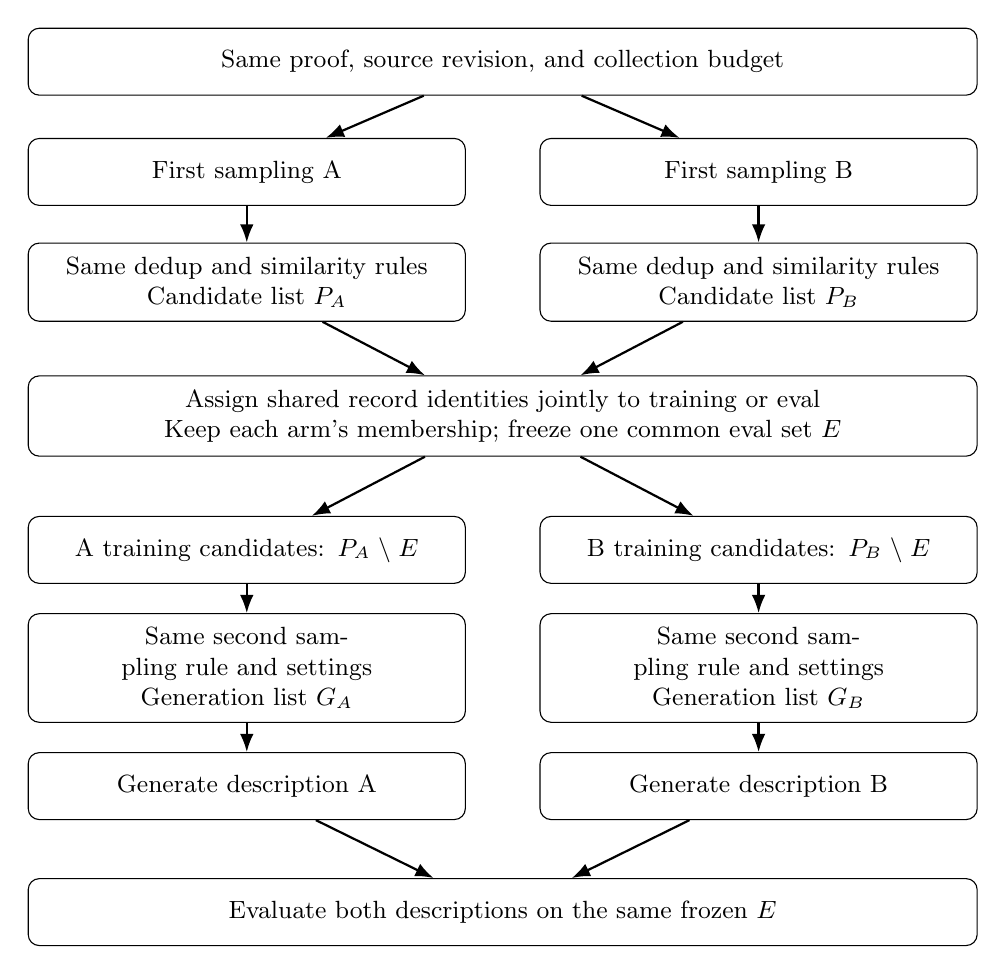
\begin{tikzpicture}[
  >=Latex,
  flow/.style={->, thick},
  box/.style={draw, rounded corners, align=center, text width=5.2cm,
    minimum height=0.85cm, inner sep=5pt, font=\small},
  wide/.style={box, text width=11.7cm}
]
  \node[wide] (proof) at (0,0) {Same proof, source revision, and collection budget};
  \node[box] (firsta) at (-3.25,-1.4) {First sampling A};
  \node[box] (firstb) at (3.25,-1.4) {First sampling B};
  \node[box] (poola) at (-3.25,-2.8) {Same dedup and similarity rules\\Candidate list $P_A$};
  \node[box] (poolb) at (3.25,-2.8) {Same dedup and similarity rules\\Candidate list $P_B$};
  \node[wide] (split) at (0,-4.5) {Assign shared record identities jointly to training or eval\\Keep each arm's membership; freeze one common eval set $E$};
  \node[box] (traina) at (-3.25,-6.2) {A training candidates: $P_A\setminus E$};
  \node[box] (trainb) at (3.25,-6.2) {B training candidates: $P_B\setminus E$};
  \node[box] (seconda) at (-3.25,-7.7) {Same second sampling rule and settings\\Generation list $G_A$};
  \node[box] (secondb) at (3.25,-7.7) {Same second sampling rule and settings\\Generation list $G_B$};
  \node[box] (desca) at (-3.25,-9.2) {Generate description A};
  \node[box] (descb) at (3.25,-9.2) {Generate description B};
  \node[wide] (judge) at (0,-10.8) {Evaluate both descriptions on the same frozen $E$};
  \draw[flow] (proof) -- (firsta);
  \draw[flow] (proof) -- (firstb);
  \draw[flow] (firsta) -- (poola);
  \draw[flow] (firstb) -- (poolb);
  \draw[flow] (poola) -- (split);
  \draw[flow] (poolb) -- (split);
  \draw[flow] (split) -- (traina);
  \draw[flow] (split) -- (trainb);
  \draw[flow] (traina) -- (seconda);
  \draw[flow] (trainb) -- (secondb);
  \draw[flow] (seconda) -- (desca);
  \draw[flow] (secondb) -- (descb);
  \draw[flow] (desca) -- (judge);
  \draw[flow] (descb) -- (judge);
\end{tikzpicture}
\end{center}

\paragraph{一起決定歸屬，不是混合兩邊的生成資料。}
一起查看 A、B 的候選，是為了辨認內容相同的 records，\allowbreak
統一決定它們是否屬於 evaluation。
若某筆 record 被選入共同 eval set，\allowbreak 必須從兩邊的 training 候選中排除。
不能將 B 獨有的 record 加進 A，\allowbreak 或反過來補入。
A training 與 B training 可以互相重疊，\allowbreak 但任一方都不能與 eval 重疊。

例如，下列編號代表依內容辨認的 record identity，\allowbreak 而不是檔案內的行號：
\begin{quote}
$P_A=\{r_1,r_2,r_3,r_4\}$，$P_B=\{r_2,r_3,r_5,r_6\}$。\\
若選定 $E=\{r_3,r_5\}$，則\\
A training 為 $\{r_1,r_2,r_4\}$；\\
B training 為 $\{r_2,r_6\}$。
\end{quote}
兩份 descriptions 都評 $E$，\allowbreak 即使其中的 $r_5$ 原本只存在於 B 候選池。
共同 eval 不限於 A、B 的交集，\allowbreak 但每個內容 identity 只保留一份。

\paragraph{控制最後送進 LLM 的筆數。}
在相同 tactic 內，\allowbreak 對 success 與 failure 分開決定共同的生成筆數：
\[
  n_{t,o}=\min\bigl(K_{t,o},\ |T_{A,t,o}|,\ |T_{B,t,o}|\bigr),
\]
其中 $t$ 表示 tactic，\allowbreak $o$ 表示 success 或 failure，\allowbreak
$T$ 是移除 eval 後的 training 候選，\allowbreak $K$ 是預定的生成上限。
兩邊各自用相同的 deterministic 第二次 sampling 規則選出 $n_{t,o}$ 筆。
這個設計對齊的是每個 tactic 的 success／failure 總筆數，\allowbreak
不額外要求各 goal-count group 的實際筆數都相同。
相同筆數也不代表相同 token 數或 LLM 費用。
若某個 outcome 在任一邊沒有 training 候選，\allowbreak
對齊後兩邊該 outcome 都使用零筆；\allowbreak 應明確記錄此限制。

例如，若 success 上限為 40，\allowbreak
兩邊可用候選分別為 35 與 28，\allowbreak 最後各選 28 筆。
較多的一方不必刪除其餘已保存候選；\allowbreak 它們只是未用於這輪生成。
這是\textbf{固定生成筆數的比較}，\allowbreak 不是讓每種方法用盡所有可用資料的比較。

\paragraph{第一次先保留較大的候選池。}
若擔心切出 eval 後 training 太少，\allowbreak
可以在第一次 sampling 使用相同且較大的候選容量。
例如，兩邊先各保留 120 筆候選，\allowbreak
經過去重、similarity 與 eval 排除後，\allowbreak 再各選最多 40 筆 success。
這只是示例，\allowbreak 不是已決定的參數，也不保證每個 tactic 都有足夠資料。
先離線統計各階段保留量，\allowbreak 再決定容量與 eval 大小；\allowbreak
不能複製 records 湊數或將 eval 放回 training。
候選容量增加也會增加收集與儲存成本。

\subsection{情況二：比較第二次 sampling 方法}
\label{subsec:holdout-second-sampling}

第一次 sampling、dedup 與 similarity check 全部相同，\allowbreak
先取得一份共同候選池 $P$。
\textbf{在第二次 sampling 之前只切分一次}，\allowbreak
得到共同 training 候選池 $T$ 與固定 eval set $E$。
A、B 的第二次 sampling 都從同一份 $T$ 開始選。

\begin{center}
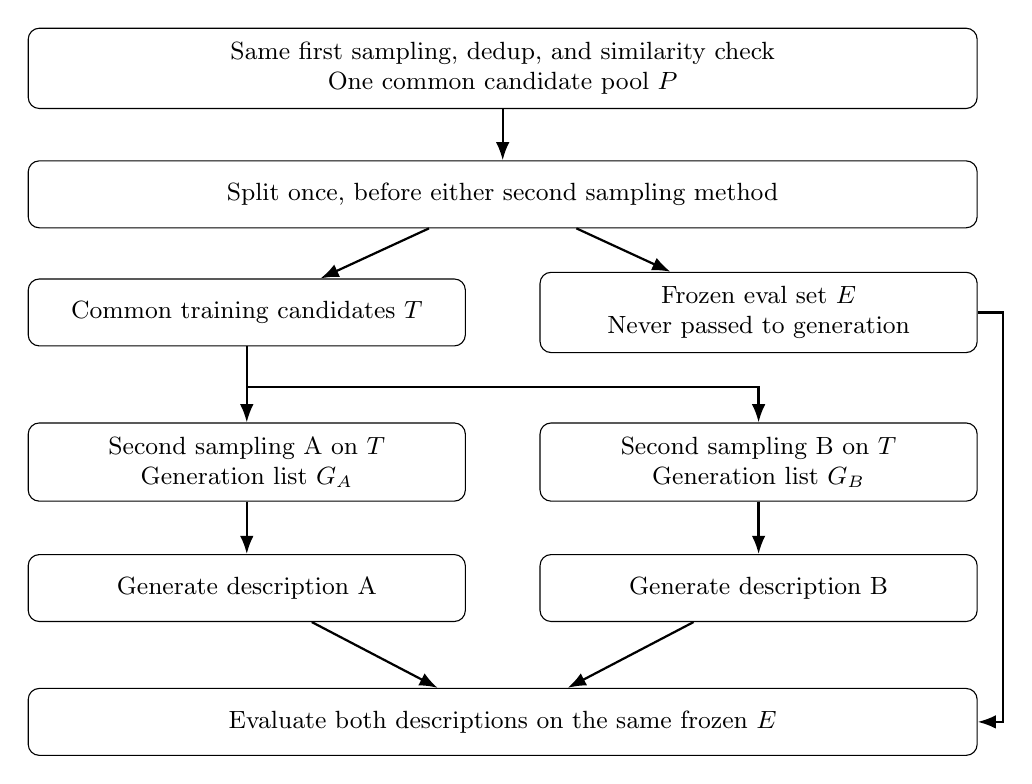
\begin{tikzpicture}[
  >=Latex,
  flow/.style={->, thick},
  box/.style={draw, rounded corners, align=center, text width=5.2cm,
    minimum height=0.85cm, inner sep=5pt, font=\small},
  wide/.style={box, text width=11.7cm}
]
  \node[wide] (pool) at (0,0) {Same first sampling, dedup, and similarity check\\One common candidate pool $P$};
  \node[wide] (split) at (0,-1.6) {Split once, before either second sampling method};
  \node[box] (training) at (-3.25,-3.1) {Common training candidates $T$};
  \node[box] (eval) at (3.25,-3.1) {Frozen eval set $E$\\Never passed to generation};
  \node[box] (seconda) at (-3.25,-5.0) {Second sampling A on $T$\\Generation list $G_A$};
  \node[box] (secondb) at (3.25,-5.0) {Second sampling B on $T$\\Generation list $G_B$};
  \node[box] (desca) at (-3.25,-6.6) {Generate description A};
  \node[box] (descb) at (3.25,-6.6) {Generate description B};
  \node[wide] (judge) at (0,-8.3) {Evaluate both descriptions on the same frozen $E$};
  \draw[flow] (pool) -- (split);
  \draw[flow] (split) -- (training);
  \draw[flow] (split) -- (eval);
  \draw[flow] (training) -- (seconda);
  \draw[flow] (training.south) -- (-3.25,-4.05) -- (3.25,-4.05) -- (secondb.north);
  \draw[flow] (seconda) -- (desca);
  \draw[flow] (secondb) -- (descb);
  \draw[flow] (desca) -- (judge);
  \draw[flow] (descb) -- (judge);
  \draw[flow] (eval.east) -- (6.35,-3.1) -- (6.35,-8.3) -- (judge.east);
\end{tikzpicture}
\end{center}

例如，共同候選池有 100 筆 success，\allowbreak
先保留 20 筆作為 eval，\allowbreak 剩下 80 筆作為 training 候選。
A、B 各自從同一份 80 筆候選選 40 筆，\allowbreak
生成兩份 descriptions，\allowbreak 然後都評同一份預留的 20 筆。
這些數字只是示意，\allowbreak failure 也需要另外規劃保留量。

不建議先執行第二次 sampling，\allowbreak
再從 A、B 的最終 lists 抽走 eval，\allowbreak 然後又 sampling 一次。
這會移除方法刻意保留的代表，\allowbreak
測到的變成兩輪選取與移除的整體效果。
若要單獨比較第二次選取方法，\allowbreak
應固定共同 training 候選、生成上限與非比較中的設定。
若某個方法因組別限制無法填滿共同目標，\allowbreak
須事先決定如何處理並記錄實際筆數，\allowbreak 不能默認兩邊一定選滿。

\subsection{兩種設計都必須遵守的規則}

令 $G_A$、$G_B$ 為實際送進 LLM 的 generation lists，\allowbreak
共同的無重疊要求為
\[
  G_A\cap E=\emptyset,\qquad G_B\cap E=\emptyset.
\]
不要求 $G_A\cap G_B=\emptyset$：\allowbreak
兩種方法可以選中相同的 training records。

\begin{enumerate}
  \item \textbf{按內容決定歸屬。}
        不能只比較檔名、proof 名稱或 record 編號。
        應依一致的內容 identity 規則辨認 records，\allowbreak
        並檢查生成與評分實際看到的 evidence 是否重複；\allowbreak
        僅來源 metadata 不同不能當成新的獨立案例。
  \item \textbf{先切分、固定，再生成與評分。}
        切分採 deterministic 規則，\allowbreak 保存 membership 與設定，\allowbreak
        不依生成結果或 judge 分數重新挑選 eval。
        切分比例、穩定排序規則、各 tactic／outcome 最低筆數仍待決定。
  \item \textbf{不足資料時明確記錄。}
        分別記錄各 tactic 的 success／failure 與 goal-count 分布。
        若沒有可評 records，\allowbreak 該項標記 N/A；\allowbreak
        若生成資料不足，\allowbreak 依事先約定的規則縮小規模或不納入，\allowbreak
        不把缺失資料當成零分。
  \item \textbf{固定生成與 judge 條件。}
        除了要比較的 sampling 方法，\allowbreak
        固定 prompt、模型、effort、token budget 與評分規則。
        兩份 descriptions 評同一份 eval evidence，\allowbreak
        分別呈現每個 tactic 的 success／failure 分數與筆數。
        Deterministic 選取不代表 LLM 回答必然相同。
  \item \textbf{保存每階段數量與來源。}
        保存 source commit、collector／selector 版本、候選設定、\allowbreak
        去重與 similarity 設定、split membership、\allowbreak
        最終 generation lists 與固定 eval set。
        報告原本可用量及最後實際使用量，\allowbreak
        避免將筆數差異誤解為內容選取的改善。
\end{enumerate}

\paragraph{解讀限制。}
這是同一批 proof records 內的 held-out evaluation，\allowbreak
不是對另一個未見 proof 的泛化測試。
完全不同的 records 也可能非常相似；\allowbreak
若需要更嚴格的分離，\allowbreak 可將相似 records 以固定共同規則分成群，\allowbreak
整群分到同一邊，\allowbreak 但此項尚未決定。
此外，切分發生在 similarity check 之後，\allowbreak
共同 eval 的分布仍受上游收集與篩選影響，\allowbreak
不能將結果直接推廣到所有 proof 執行案例。

% Needs Chinese-capable fonts, tikz, and \usetikzlibrary{arrows.meta}.
% The existing framework.tex already provides these prerequisites.

\section{比較兩階段 sampling 時的 training 與 evaluation 切分}
\label{sec:sampling-training-evaluation-workflows}

本節記錄預定的實驗設計，\allowbreak 不代表已經實作或執行。
這裡的 training records 是提供給 LLM 生成 description 的範例，\allowbreak
不會訓練或更新模型權重。
為避免混淆，\allowbreak 下文區分「training 候選池」與「最後送進 LLM 的 generation list」。

\begin{itemize}
  \item \textbf{第一次 sampling：}collector 在 proof 執行時選取並保留候選 records。
  \item \textbf{中間處理：}依既定流程合併候選、exact dedup 與 similarity check。
  \item \textbf{第二次 sampling：}從候選池依分組配額與遞補規則，\allowbreak
        選出最後用來生成 description 的 records。
\end{itemize}

\subsection{情況一：比較第一次 sampling 方法}
\label{subsec:holdout-first-sampling}

A、B 從相同 proof 與 source commit 開始，\allowbreak
使用不同的第一次 sampling 方法。
兩邊使用相同候選容量，\allowbreak 並固定其餘 collector 設定、dedup 與 similarity check 規則。
因此，中間處理後的候選 lists 可以不同，\allowbreak 這正是要保留的實驗差異。

\begin{center}
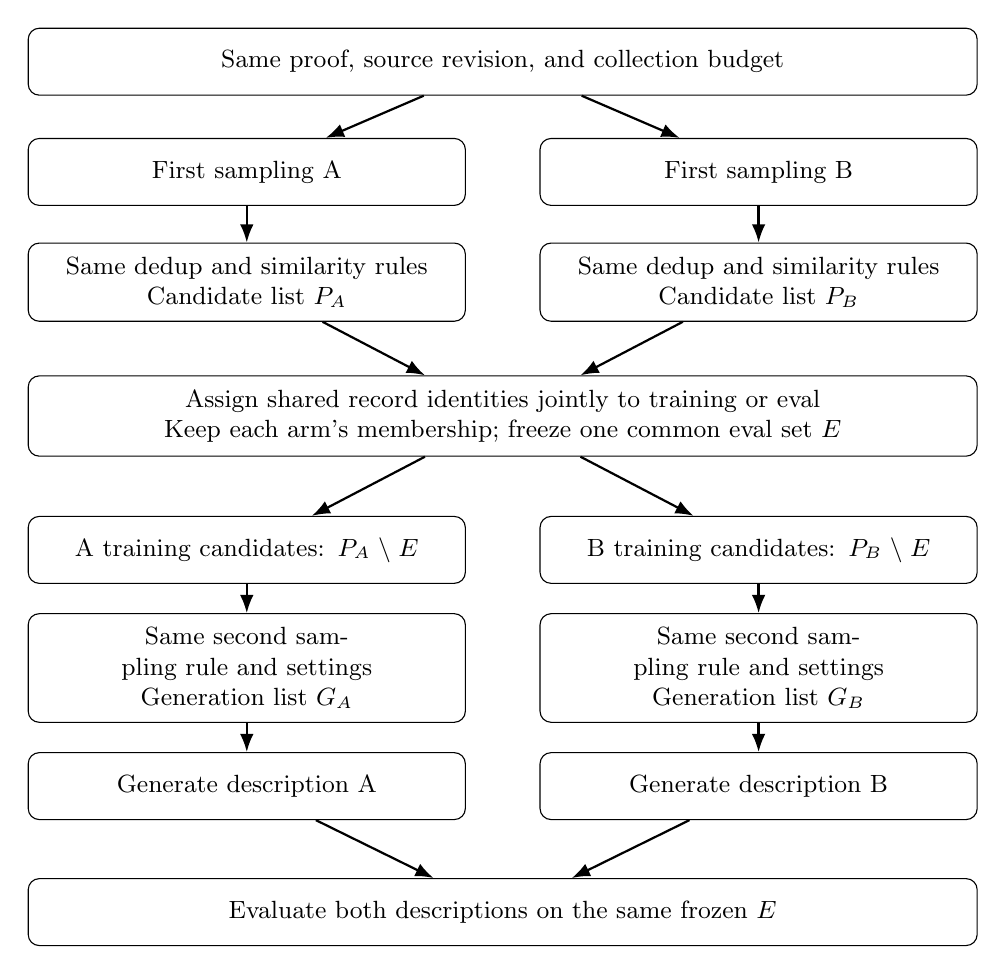
\begin{tikzpicture}[
  >=Latex,
  flow/.style={->, thick},
  box/.style={draw, rounded corners, align=center, text width=5.2cm,
    minimum height=0.85cm, inner sep=5pt, font=\small},
  wide/.style={box, text width=11.7cm}
]
  \node[wide] (proof) at (0,0) {Same proof, source revision, and collection budget};
  \node[box] (firsta) at (-3.25,-1.4) {First sampling A};
  \node[box] (firstb) at (3.25,-1.4) {First sampling B};
  \node[box] (poola) at (-3.25,-2.8) {Same dedup and similarity rules\\Candidate list $P_A$};
  \node[box] (poolb) at (3.25,-2.8) {Same dedup and similarity rules\\Candidate list $P_B$};
  \node[wide] (split) at (0,-4.5) {Assign shared record identities jointly to training or eval\\Keep each arm's membership; freeze one common eval set $E$};
  \node[box] (traina) at (-3.25,-6.2) {A training candidates: $P_A\setminus E$};
  \node[box] (trainb) at (3.25,-6.2) {B training candidates: $P_B\setminus E$};
  \node[box] (seconda) at (-3.25,-7.7) {Same second sampling rule and settings\\Generation list $G_A$};
  \node[box] (secondb) at (3.25,-7.7) {Same second sampling rule and settings\\Generation list $G_B$};
  \node[box] (desca) at (-3.25,-9.2) {Generate description A};
  \node[box] (descb) at (3.25,-9.2) {Generate description B};
  \node[wide] (judge) at (0,-10.8) {Evaluate both descriptions on the same frozen $E$};
  \draw[flow] (proof) -- (firsta);
  \draw[flow] (proof) -- (firstb);
  \draw[flow] (firsta) -- (poola);
  \draw[flow] (firstb) -- (poolb);
  \draw[flow] (poola) -- (split);
  \draw[flow] (poolb) -- (split);
  \draw[flow] (split) -- (traina);
  \draw[flow] (split) -- (trainb);
  \draw[flow] (traina) -- (seconda);
  \draw[flow] (trainb) -- (secondb);
  \draw[flow] (seconda) -- (desca);
  \draw[flow] (secondb) -- (descb);
  \draw[flow] (desca) -- (judge);
  \draw[flow] (descb) -- (judge);
\end{tikzpicture}
\end{center}

\paragraph{一起決定歸屬，不是混合兩邊的生成資料。}
一起查看 A、B 的候選，是為了辨認內容相同的 records，\allowbreak
統一決定它們是否屬於 evaluation。
若某筆 record 被選入共同 eval set，\allowbreak 必須從兩邊的 training 候選中排除。
不能將 B 獨有的 record 加進 A，\allowbreak 或反過來補入。
A training 與 B training 可以互相重疊，\allowbreak 但任一方都不能與 eval 重疊。

例如，下列編號代表依內容辨認的 record identity，\allowbreak 而不是檔案內的行號：
\begin{quote}
$P_A=\{r_1,r_2,r_3,r_4\}$，$P_B=\{r_2,r_3,r_5,r_6\}$。\\
若選定 $E=\{r_3,r_5\}$，則\\
A training 為 $\{r_1,r_2,r_4\}$；\\
B training 為 $\{r_2,r_6\}$。
\end{quote}
兩份 descriptions 都評 $E$，\allowbreak 即使其中的 $r_5$ 原本只存在於 B 候選池。
共同 eval 不限於 A、B 的交集，\allowbreak 但每個內容 identity 只保留一份。

\paragraph{控制最後送進 LLM 的筆數。}
在相同 tactic 內，\allowbreak 對 success 與 failure 分開決定共同的生成筆數：
\[
  n_{t,o}=\min\bigl(K_{t,o},\ |T_{A,t,o}|,\ |T_{B,t,o}|\bigr),
\]
其中 $t$ 表示 tactic，\allowbreak $o$ 表示 success 或 failure，\allowbreak
$T$ 是移除 eval 後的 training 候選，\allowbreak $K$ 是預定的生成上限。
兩邊各自用相同的 deterministic 第二次 sampling 規則選出 $n_{t,o}$ 筆。
這個設計對齊的是每個 tactic 的 success／failure 總筆數，\allowbreak
不額外要求各 goal-count group 的實際筆數都相同。
相同筆數也不代表相同 token 數或 LLM 費用。
若某個 outcome 在任一邊沒有 training 候選，\allowbreak
對齊後兩邊該 outcome 都使用零筆；\allowbreak 應明確記錄此限制。

例如，若 success 上限為 40，\allowbreak
兩邊可用候選分別為 35 與 28，\allowbreak 最後各選 28 筆。
較多的一方不必刪除其餘已保存候選；\allowbreak 它們只是未用於這輪生成。
這是\textbf{固定生成筆數的比較}，\allowbreak 不是讓每種方法用盡所有可用資料的比較。

\paragraph{第一次先保留較大的候選池。}
若擔心切出 eval 後 training 太少，\allowbreak
可以在第一次 sampling 使用相同且較大的候選容量。
例如，兩邊先各保留 120 筆候選，\allowbreak
經過去重、similarity 與 eval 排除後，\allowbreak 再各選最多 40 筆 success。
這只是示例，\allowbreak 不是已決定的參數，也不保證每個 tactic 都有足夠資料。
先離線統計各階段保留量，\allowbreak 再決定容量與 eval 大小；\allowbreak
不能複製 records 湊數或將 eval 放回 training。
候選容量增加也會增加收集與儲存成本。

\subsection{情況二：比較第二次 sampling 方法}
\label{subsec:holdout-second-sampling}

第一次 sampling、dedup 與 similarity check 全部相同，\allowbreak
先取得一份共同候選池 $P$。
\textbf{在第二次 sampling 之前只切分一次}，\allowbreak
得到共同 training 候選池 $T$ 與固定 eval set $E$。
A、B 的第二次 sampling 都從同一份 $T$ 開始選。

\begin{center}
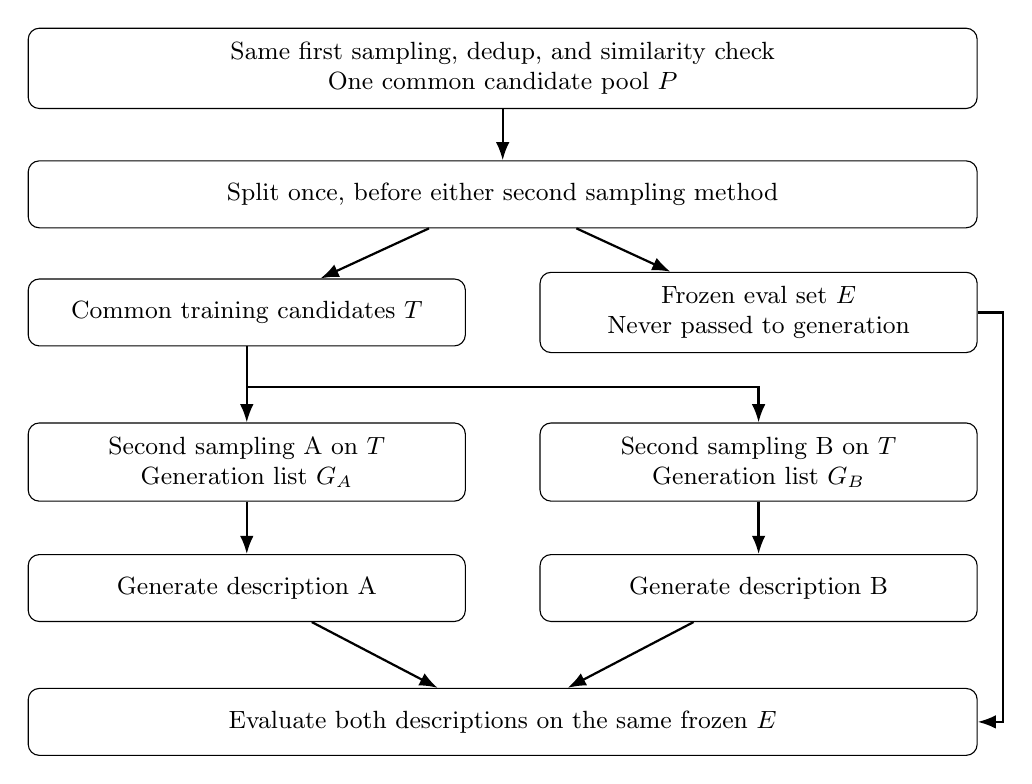
\begin{tikzpicture}[
  >=Latex,
  flow/.style={->, thick},
  box/.style={draw, rounded corners, align=center, text width=5.2cm,
    minimum height=0.85cm, inner sep=5pt, font=\small},
  wide/.style={box, text width=11.7cm}
]
  \node[wide] (pool) at (0,0) {Same first sampling, dedup, and similarity check\\One common candidate pool $P$};
  \node[wide] (split) at (0,-1.6) {Split once, before either second sampling method};
  \node[box] (training) at (-3.25,-3.1) {Common training candidates $T$};
  \node[box] (eval) at (3.25,-3.1) {Frozen eval set $E$\\Never passed to generation};
  \node[box] (seconda) at (-3.25,-5.0) {Second sampling A on $T$\\Generation list $G_A$};
  \node[box] (secondb) at (3.25,-5.0) {Second sampling B on $T$\\Generation list $G_B$};
  \node[box] (desca) at (-3.25,-6.6) {Generate description A};
  \node[box] (descb) at (3.25,-6.6) {Generate description B};
  \node[wide] (judge) at (0,-8.3) {Evaluate both descriptions on the same frozen $E$};
  \draw[flow] (pool) -- (split);
  \draw[flow] (split) -- (training);
  \draw[flow] (split) -- (eval);
  \draw[flow] (training) -- (seconda);
  \draw[flow] (training.south) -- (-3.25,-4.05) -- (3.25,-4.05) -- (secondb.north);
  \draw[flow] (seconda) -- (desca);
  \draw[flow] (secondb) -- (descb);
  \draw[flow] (desca) -- (judge);
  \draw[flow] (descb) -- (judge);
  \draw[flow] (eval.east) -- (6.35,-3.1) -- (6.35,-8.3) -- (judge.east);
\end{tikzpicture}
\end{center}

例如，共同候選池有 100 筆 success，\allowbreak
先保留 20 筆作為 eval，\allowbreak 剩下 80 筆作為 training 候選。
A、B 各自從同一份 80 筆候選選 40 筆，\allowbreak
生成兩份 descriptions，\allowbreak 然後都評同一份預留的 20 筆。
這些數字只是示意，\allowbreak failure 也需要另外規劃保留量。

不建議先執行第二次 sampling，\allowbreak
再從 A、B 的最終 lists 抽走 eval，\allowbreak 然後又 sampling 一次。
這會移除方法刻意保留的代表，\allowbreak
測到的變成兩輪選取與移除的整體效果。
若要單獨比較第二次選取方法，\allowbreak
應固定共同 training 候選、生成上限與非比較中的設定。
若某個方法因組別限制無法填滿共同目標，\allowbreak
須事先決定如何處理並記錄實際筆數，\allowbreak 不能默認兩邊一定選滿。

\subsection{兩種設計都必須遵守的規則}

令 $G_A$、$G_B$ 為實際送進 LLM 的 generation lists，\allowbreak
共同的無重疊要求為
\[
  G_A\cap E=\emptyset,\qquad G_B\cap E=\emptyset.
\]
不要求 $G_A\cap G_B=\emptyset$：\allowbreak
兩種方法可以選中相同的 training records。

\begin{enumerate}
  \item \textbf{按內容決定歸屬。}
        不能只比較檔名、proof 名稱或 record 編號。
        應依一致的內容 identity 規則辨認 records，\allowbreak
        並檢查生成與評分實際看到的 evidence 是否重複；\allowbreak
        僅來源 metadata 不同不能當成新的獨立案例。
  \item \textbf{先切分、固定，再生成與評分。}
        切分採 deterministic 規則，\allowbreak 保存 membership 與設定，\allowbreak
        不依生成結果或 judge 分數重新挑選 eval。
        切分比例、穩定排序規則、各 tactic／outcome 最低筆數仍待決定。
  \item \textbf{不足資料時明確記錄。}
        分別記錄各 tactic 的 success／failure 與 goal-count 分布。
        若沒有可評 records，\allowbreak 該項標記 N/A；\allowbreak
        若生成資料不足，\allowbreak 依事先約定的規則縮小規模或不納入，\allowbreak
        不把缺失資料當成零分。
  \item \textbf{固定生成與 judge 條件。}
        除了要比較的 sampling 方法，\allowbreak
        固定 prompt、模型、effort、token budget 與評分規則。
        兩份 descriptions 評同一份 eval evidence，\allowbreak
        分別呈現每個 tactic 的 success／failure 分數與筆數。
        Deterministic 選取不代表 LLM 回答必然相同。
  \item \textbf{保存每階段數量與來源。}
        保存 source commit、collector／selector 版本、候選設定、\allowbreak
        去重與 similarity 設定、split membership、\allowbreak
        最終 generation lists 與固定 eval set。
        報告原本可用量及最後實際使用量，\allowbreak
        避免將筆數差異誤解為內容選取的改善。
\end{enumerate}

\paragraph{解讀限制。}
這是同一批 proof records 內的 held-out evaluation，\allowbreak
不是對另一個未見 proof 的泛化測試。
完全不同的 records 也可能非常相似；\allowbreak
若需要更嚴格的分離，\allowbreak 可將相似 records 以固定共同規則分成群，\allowbreak
整群分到同一邊，\allowbreak 但此項尚未決定。
此外，切分發生在 similarity check 之後，\allowbreak
共同 eval 的分布仍受上游收集與篩選影響，\allowbreak
不能將結果直接推廣到所有 proof 執行案例。

% Current execution-time C workflow, checked against source on 2026-10-16.
% Section fragment; uses the existing tikz and arrows.meta setup in main.tex.
% This documents behavior and constraints, not a completed proof experiment.

\section{在 proof 執行時收集獨立隨機 evaluation set C}
\label{sec:independent-random-evaluation-workflow}

本節說明另一種已實作的資料收集流程：\allowbreak
在 proof 執行時，\allowbreak 從符合條件的 tactic applications 另外抽出 evaluation set $C$。
這裡的「獨立」指抽樣途徑不依賴 generation sampler 的保留結果，\allowbreak
不表示 $C$ 與生成資料必然沒有重疊。
本節依目前程式與文件說明流程，\allowbreak 不代表已完成完整 proof 實驗或 description 品質評估。

\subsection{先分流，再分別建立生成資料與 C}

\textbf{$C$ 的分流發生在 generation sampling、dedup 與 similarity check 之前。}
每次被 instrumentation 記錄的 tactic application，\allowbreak
通過共同的大小與 assumption 數量限制後，\allowbreak
同時可進入 generation 路徑與獨立的 random reservoir。
因此，即使某筆 record 後來沒有被 generation sampler 保留，\allowbreak
它仍有機會進入 $C$。
若只從已保存的 generation records 離線再抽樣，\allowbreak
就無法找回執行時已丟棄的 records，\allowbreak 因而不是這裡的流程。

\begin{center}
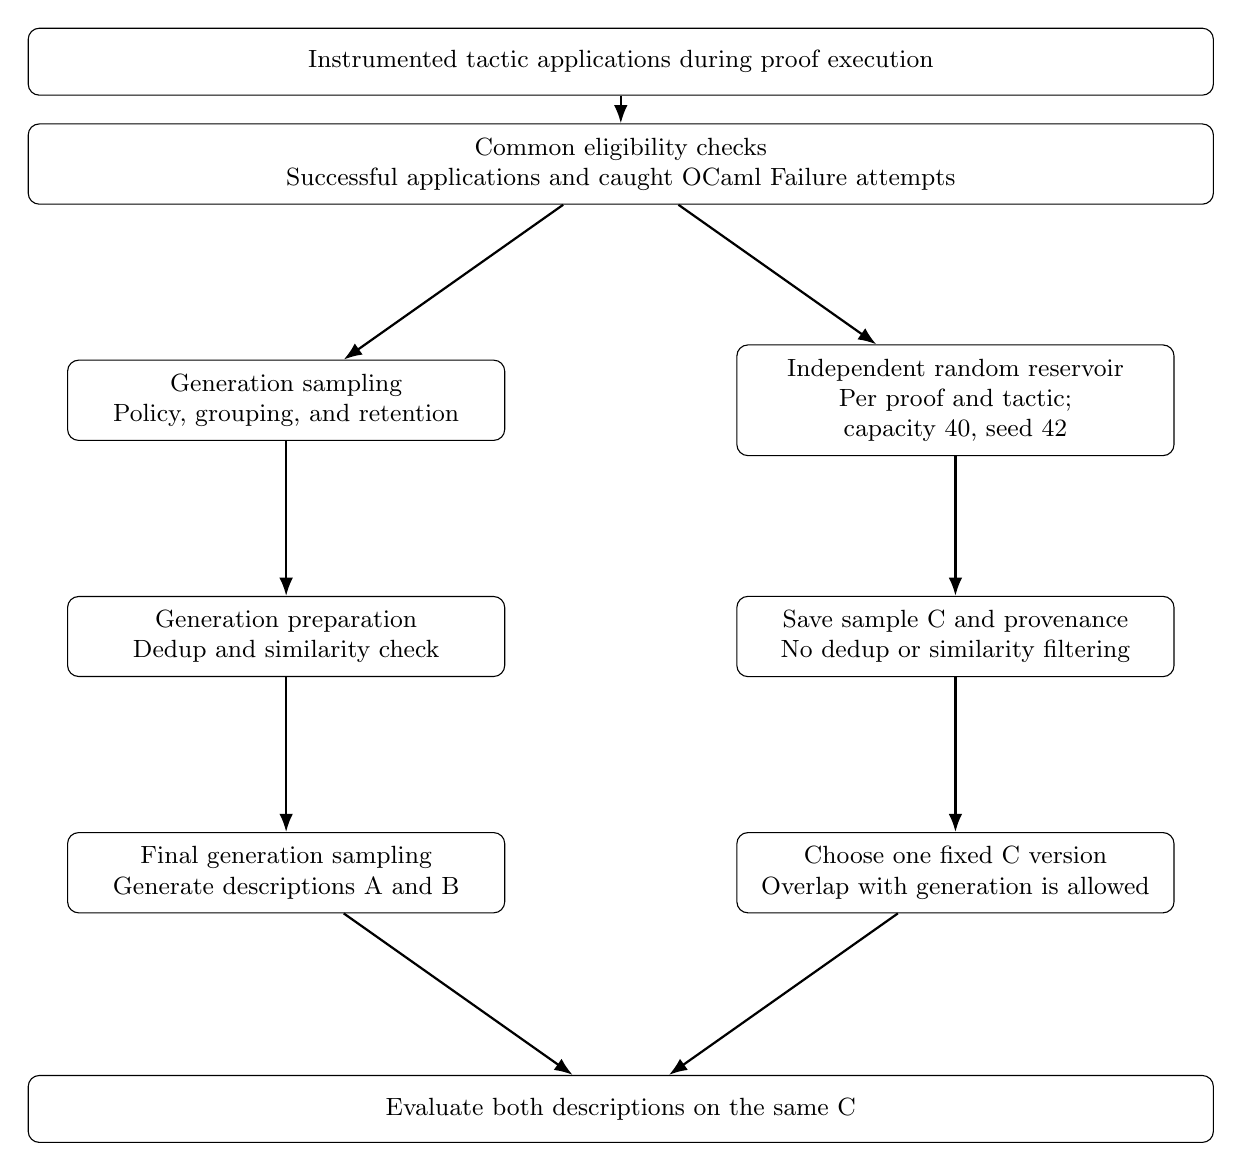
\begin{tikzpicture}[
  >=Latex,
  flow/.style={->, thick},
  box/.style={draw, rounded corners, align=center, text width=5.2cm,
    minimum height=0.85cm, inner sep=5pt, font=\small},
  wide/.style={box, text width=14.7cm}
]
  \node[wide] (stream) at (0,0) {Instrumented tactic applications during proof execution};
  \node[wide] (eligible) at (0,-1.3) {Common eligibility checks\\Successful applications and caught OCaml Failure attempts};
  \node[box] (generation) at (-4.25,-4.3) {Generation sampling\\Policy, grouping, and retention};
  \node[box] (reservoir) at (4.25,-4.3) {Independent random reservoir\\Per proof and tactic; capacity 40, seed 42};
  \node[box] (prepare) at (-4.25,-7.3) {Generation preparation\\Dedup and similarity check};
  \node[box] (samplec) at (4.25,-7.3) {Save sample C and provenance\\No dedup or similarity filtering};
  \node[box] (descriptions) at (-4.25,-10.3) {Final generation sampling\\Generate descriptions A and B};
  \node[box] (freeze) at (4.25,-10.3) {Choose one fixed C version\\Overlap with generation is allowed};
  \node[wide] (judge) at (0,-13.3) {Evaluate both descriptions on the same C};
  \draw[flow] (stream) -- (eligible);
  \draw[flow] (eligible) -- (generation);
  \draw[flow] (eligible) -- (reservoir);
  \draw[flow] (generation) -- (prepare);
  \draw[flow] (reservoir) -- (samplec);
  \draw[flow] (prepare) -- (descriptions);
  \draw[flow] (samplec) -- (freeze);
  \draw[flow] (descriptions) -- (judge);
  \draw[flow] (freeze) -- (judge);
\end{tikzpicture}
\end{center}

圖中左側代表 A、B 各自的生成流程；\allowbreak
要比較第一次 sampling 時可使用不同 collector policy，\allowbreak
比較第二次 sampling 時則固定共同候選池。
右側的 $C$ 不從 A、B 的最終 generation lists 選取，\allowbreak
兩份 descriptions 必須使用同一版本的 $C$ 評分。

\paragraph{哪些 applications 會進入 C？}
成功的 tactic applications 與被捕捉為 OCaml \texttt{Failure} 的失敗嘗試都可納入，\allowbreak
包括成功 proof 中途試過但失敗的 tactic。
Conversions 與其他種類的 exceptions 不當成這裡的 tactic failure。
共同 eligibility 限制仍然存在，\allowbreak
因此 $C$ 代表符合條件且有 instrumentation 的 applications，\allowbreak
不能視為所有 proof states 或 HOL Light 所有操作的完整樣本。

\paragraph{抽樣單位與預設設定。}
每個 proof execution 的每個 tactic 各有一個 random reservoir，\allowbreak
預設最多保留 40 筆，\allowbreak independent seed 為 42。
Success 與 failure 共用這 40 筆容量，\allowbreak
不按 outcome 或 goal count 設配額，\allowbreak 所以不保證兩種 outcome 都有樣本。
每次出現算一個 occurrence：\allowbreak
內容相同的兩次呼叫仍是兩次抽樣機會，\allowbreak 也可能同時被保留。
相同 seed 與相同順序的 eligible stream 可重現選取結果；\allowbreak
執行順序改變則結果可能改變。
不同 proofs 使用相同 seed，\allowbreak 也不保證它們的抽樣在統計上彼此獨立。

\paragraph{這不是 held-out evaluation。}
本節允許 $G_A\cap C$ 或 $G_B\cap C$ 非空，\allowbreak
其中 $G_A$、$G_B$ 是實際用於生成 descriptions 的 records。
不要因為重疊而補抽或移除 $C$，\allowbreak 否則會改變原先的抽樣分布。
有保存實際 generation requests 時，\allowbreak 可以量測並回報 overlap。
前一節要求 generation 與 eval 無重疊，\allowbreak
本節則評估固定 eligible stream 樣本上的表現；\allowbreak
兩種設計的評分意義不同，\allowbreak 不能將本節結果稱為未見 records 的泛化表現。

\subsection{日常執行：自動沿用，或收集新的 C}

日常 sampling workflow 與新建立的 experiment config 預設使用 \texttt{auto}。
檢查發生在啟動實驗時，\allowbreak
依經過驗證的 build 所使用的 source 決定能否沿用 $C$；\allowbreak
既有 pinned-source 設定仍決定實際執行哪個版本。
這不是背景檔案監看器，\allowbreak 修改或新增 \texttt{.ml} 檔案本身不會立刻觸發收集。

\begin{itemize}
  \item \textbf{auto：}找到來源與獨立抽樣設定相符、且通過驗證的 sample 時沿用；\allowbreak
        新 proof 或相關 inputs 改變、沒有相符 sample 時，\allowbreak 在 proof 執行中收集新的 $C$。
        沿用 $C$ 時 generation 的 proof execution 仍會執行，\allowbreak
        只是該 proof 的獨立 collector 關閉。
  \item \textbf{on：}強制在這次新的 proof execution 收集，\allowbreak
        適合需要目前 source revision 對應資料的情況。
  \item \textbf{off：}這次執行不收集也不沿用 $C$。
        Independent capacity 設為零時，\allowbreak 在所有模式下都停用此功能。
\end{itemize}

是否能沿用，\allowbreak 不只檢查最外層 proof \texttt{.ml}：\allowbreak
還包含展開後的 source dependencies、HOL source、\allowbreak
proof 以 literal 路徑引用的 object files，\allowbreak 以及獨立抽樣的規則、capacity 與 seed。
程式不推測執行時才計算出的 object 路徑。
只改 generation policy、分組、配額、filtering、最終選取或 description prompt，\allowbreak
本身不要求重抽 $C$；\allowbreak unrelated proof 的新增 object 也不會使此 sample 失效。
Independent seed 與 generation 的 \texttt{--seed} 分開設定。

手動覆寫可使用 \dpath{--independent-eval-mode}、\allowbreak
\dpath{--independent-eval-capacity} 與 \dpath{--independent-eval-seed}。
較底層的 \dpath{scripts/run-with-sampling.sh} 仍是手動流程，\allowbreak
不會自動搜尋或發布可沿用的 $C$；\allowbreak
舊的 explicit capacity／seed configs 也保留原有手動行為。
歷史 schema-v1 configs 除非明確啟用，\allowbreak 否則維持停用。
新的 collector 與 runtime adapter 必須編入 executable；\allowbreak
只更新腳本不會更新既有 \texttt{.native}。

\subsection{保存版本、新增 proof，以及評分時的來源限制}

Collector 將 records 與 metadata 分別寫到\allowbreak
\dpath{PROOF.ml.independent-eval/TAC.json} 與\allowbreak
\dpath{PROOF.ml.independent-eval.json}。
Metadata 保存 seed、capacity、eligible／retained 數量與選中 occurrence 的位置，\allowbreak
workflow 再附上 build 與 source provenance。
這些 records 不會進入一般 generation preparation。

自動流程在本機為每個 proof 保存一份可驗證的 sample，\allowbreak
並在 collection receipt 的 \dpath{independent_eval.reference} 記錄引用。
發布檔案位於 dataset root 的 \dpath{data/evaluation/} 與\allowbreak
\dpath{data/metadata/}；\allowbreak 這個動作不會上傳 Hugging Face。
改變來源後產生新 sample，\allowbreak 舊版本與原始 provenance 都保留。
沿用舊 sample 也不會把它的 source commit 改寫成新 commit。

\paragraph{新增 proof 不會自動合併成一份全域 C。}
將新 proof 加入選取清單後，\allowbreak
\texttt{auto} 可沿用未變更 proofs 的 samples，\allowbreak
並收集新 proof 中既有與新出現 tactics 的樣本。
各 proof references 仍然分開；\allowbreak
需要共同評分集合時，\allowbreak 使用手動 publisher 明確合併指定 samples。
可用 \dpath{--previous-manifest} 保留舊 samples 並加入新 proof，\allowbreak
建立新的 $C$ 版本，\allowbreak 不覆寫舊版本也不再隨機抽一次。
同一 proof、同一 source version 的重複匯入會被拒絕。
A、B 必須一起改用相同的新版本。

這是逐 proof、逐 tactic 抽樣後的累積，\allowbreak
不是把所有 proofs 的 occurrences 合在一起均勻抽樣。
例如，同一 tactic 在兩個 proofs 各有 20 與 200 個 eligible occurrences，\allowbreak
capacity 40 時前者全留，\allowbreak 後者只留 40 筆，\allowbreak
兩邊單筆 occurrence 的入選機率不同。
報告分數時應一併列出 proof 清單、版本、各 tactic 的筆數與 outcome coverage。

\paragraph{沿用判斷與 judge 的 commit 檢查不同。}
來源內容相同時，\allowbreak 自動流程可能跨 Git commits 沿用 sample，\allowbreak
但目前 judge 要求 $C$ 與兩份 description setups 共用同一個已知 source commit。
因此跨 commit 沿用的 sample 仍可能被 judge 拒絕。
需要對齊時，\allowbreak 使用 \texttt{on} 在所需 revision 收集，\allowbreak
再手動發布這次輸出；\allowbreak 合併評分用 proofs 也應來自同一 revision。
保留 raw samples、build receipts 與 manifests，\allowbreak
不要為通過檢查而改寫舊資料的來源。

\end{document}